\documentclass[11pt]{article}
\usepackage[paperwidth=12cm, paperheight=18cm, margin=1cm]{geometry}
\usepackage{amsmath, tikz}
\pagestyle{empty}

\begin{document}
\begin{center}
  {\LARGE\bfseries The Monty Hall Problem}\\[4pt]
  {\large Should you switch doors?}
\end{center}

Three doors: one car, two goats. You pick a door. The host,
who knows where the car is, opens another door with a goat
and offers you the chance to switch.

\section*{Sticking wins only if your first pick was right}
\[
  P(\text{win} \mid \text{stick}) = \frac{1}{3}
\]

\section*{Switching wins whenever your first pick was wrong}
\[
  P(\text{win} \mid \text{switch}) = 1 - \frac{1}{3} = \frac{2}{3}
\]

\begin{center}
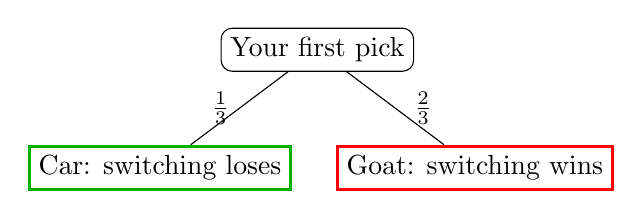
\begin{tikzpicture}[level distance=1.5cm, sibling distance=4cm]
  \node[draw, rounded corners] {Your first pick}
    child {node[draw=green!70!black, very thick] {Car: switching loses}
      edge from parent node[left] {$\tfrac13$\ }}
    child {node[draw=red, very thick] {Goat: switching wins}
      edge from parent node[right] {\ $\tfrac23$}};
\end{tikzpicture}
\end{center}

\begin{center}
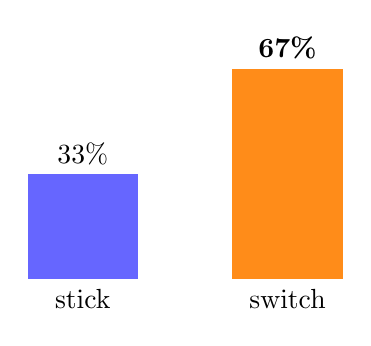
\begin{tikzpicture}
  \fill[blue!60] (0,0) rectangle (1.4,1.33);
  \fill[orange!90] (2.6,0) rectangle (4,2.67);
  \node[above] at (0.7,1.33) {33\%};
  \node[above] at (3.3,2.67) {\bfseries 67\%};
  \node[below] at (0.7,0) {stick};
  \node[below] at (3.3,0) {switch};
\end{tikzpicture}
\end{center}

\centerline{\bfseries Always switch: it doubles your chances.}
\end{document}
